\section{Mock data}\label{sec:mocks}

We apply our method to a set of mock data,
consisting of multiple tracers moving in spherical
or triaxial potentials with radial or tangential
velocity anisotropy. All mock data are available
on the {\sc Gaia Challenge} wiki
site\footnote{\href{http://astrowiki.ph.surrey.ac.uk/dokuwiki/}{http://astrowiki.ph.surrey.ac.uk/dokuwiki/}}. The
first set of mocks have cusped or cored dark
matter density profiles with radial anisotropy --
the `Walker' mocks (WP11), with tracer density:

\begin{equation}
    \nu_*(r) = \nu_0\left(\frac{r}{r_*}\right)^{-\gamma_*} \left[1+\left(\frac{r}{r_*}\right)^{\alpha_*}\right]^{(\gamma_*-\beta_*)/\alpha_*}
\end{equation}
inside dark matter halos of the form:

\begin{equation}
    \rho_{\text{DM}} = \rho_0\left(\frac{r}{r_{\text{DM}}}\right)^{-\gamma_{\text{DM}}}\left[1+\left(\frac{r}{r_{\text{DM}}}\right)^{\alpha_{\text{DM}}}\right]^{(\gamma_{\text{DM}}-\beta_{\text{DM}})/\alpha_{\text{DM}}}
\end{equation}
with scale radii $r_*, r_\text{DM}$; central
slopes of $\gamma_*, \gamma_{\text{DM}}$;
transition parameters $\beta_*,\beta_{\text{DM}}$;
and outer slopes $\alpha_*, \alpha_{\text{DM}}$.

The anisotropy follows the functional form of
\citet{Osipkov1979} and \citet{Merritt1985}:

\begin{equation}
    \beta(r)=1-\frac{\sigma_\theta^2}{\sigma_r^2} = \frac{r^2}{r^2+r_a^2}.
\end{equation}
with scale radius $r_a$, turning over from nearly
isotropic at $r\to 0$ to radially biased at
$r_*=r_a$.

Of these distributions, finite samplings are
taken, giving our first set of mock data, table
\ref{tab:gaia}, and then converted to mock
observational data including observational
parameters like spectral indices, systemic
velocities, proper motions, and binary
motions. The full suite of mock data is much
larger than that used here. Our particular subset
is given in table \ref{tab:walk}.

In addition to the above Walker mocks, we add also
a mock dwarf with cusped triaxial model viewed
along three different projection angles: down the
minor axis; the major axis; and the intermediate
axis. All models are summarised in Table
\ref{tab:triax}.

\begin{table}
    \label{tab:gaia}
    \caption{Parameters of the 1-population Gaia challenge mock data.}
    \centering
    \begin{tabular}{lllll}
        ID & geometry & $\gamma_{\text{DM}}$ & $\gamma_*$ & $r_*$\\
        \hline
        Gaia01 & sphere & 1 & 0.1 & 100 pc\\
        Gaia02 & sphere & 0 & 0.1 & 250 pc\\
        Gaia03 & sphere & 1 & 0.1 & 250 pc\\
        Gaia04 & sphere & 0 & 0.1 & 1000 pc\\
        Gaia05 & sphere & 1 & 1.0 & 100 pc\\
        Gaia06 & sphere & 0 & 1.0 & 250 pc\\
        Gaia07 & sphere & 1 & 1.0 & 250 pc\\
        Gaia08 & sphere & 0 & 1.0 & 1000 pc\\
        Gaia09 & sphere & TODO & TODO & TODO pc\\
        Gaia10 & sphere & TODO & TODO & TODO pc\\
        Gaia11 & sphere, tangential & 1 & 1.0 & 500 pc\\
        Gaia12 & sphere, tangential & 0 & 1.0 & 1750 pc\\\hline\hline
    \end{tabular}
\end{table}

\begin{table}
    \label{tab:walk}
    \caption{Parameters of the 2-population Walker mock data.}
    \centering
    \begin{tabular}{llll}
        ID & geometry & $\gamma_{\text{DM}}$ & $r_{1/2,\text{DM}}$\\
        \hline
        Walk01 & sphere & 0 & 1000 pc \\
        Walk02 & sphere & 1 & 1000 pc\\\hline\hline
    \end{tabular}
\end{table}

\begin{table}
    \label{tab:triax}
    \caption{Parameters of the 1-population triaxial mock data.}
    \centering
    \begin{tabular}{lll}
        ID & geometry & $\gamma_DM$\\
        \hline
        Triax01 & triaxial, intermediate axis & 0\\
        Triax02 & triaxial, along x & 0 \\
        Triax03 & triaxial, along y & 0 \\
        Triax04 & triaxial, along z & 0 \\
        Triax05 & triaxial, intermediate axis & 1\\
        Triax06 & triaxial, along x & 1\\
        Triax07 & triaxial, along y & 1\\
        Triax08 & triaxial, along z & 1\\\hline\hline
    \end{tabular}
\end{table}

\section{Results}\label{sec:results}
\subsection{Single tracer population}
We first apply our method to DM halos hosting a single population of
tracer stars. We consider both cored and cusped models. As default, we
assume that we have 10,000 tracer stars. We consider poorer sampling
in \S\ref{sec:sampling}. The cusped model has: $\gamma_{DM}=1$,
stellar central density slope $\gamma_{*,1}=0.1, \gamma_{*,2}=0.1$;
stellar turnover slopes $\beta_{*,1}=\beta_{*,2}=5$; stellar
characteristic radii $r_{*,1}=100\pc, r_{*,2}=500\pc$; and anisotropy
scale radii $r_{a,1}=r_{a,2}=1.0$. All other parameters are as in
table \ref{tab:gaia}. Our results for the recovered mass distributions
are shown in Figure \ref{fig:singlepop}; Figure
\ref{fig:Sigsiglos1pop} shows a comparison of the model tracer surface
density $\Sigma(r)$ and projected velocity dispersion $\siglos(r)$
with mock data for the cusped case. Notice that in all cases, we
successfully recover the input model within our quoted uncertainties.


\begin{figure*}
    \begin{center}
        % cored profile
        \includegraphics[width=0.33\textwidth]{fig/Gaia02/output/pdf/prof_rho_0}\hspace{-3mm}
        \includegraphics[width=0.33\textwidth]{fig/Gaia02/output/pdf/prof_nr_0}\hspace{-3mm}
        \includegraphics[width=0.33\textwidth]{fig/Gaia02/output/pdf/prof_betastar_1}

        % cusped profile
        \includegraphics[width=0.33\textwidth]{fig/Gaia03/output/pdf/prof_rho_0}\hspace{-3mm}
        \includegraphics[width=0.33\textwidth]{fig/Gaia03/output/pdf/prof_nr_0}\hspace{-3mm}
        \includegraphics[width=0.33\textwidth]{fig/Gaia03/output/pdf/prof_betastar_1}

        \caption{Reconstructed density for Gaia02
          (cored, top), and Gaia03 (cusped,
          bottom); logarithmic density slope; and
          velocity anisotropy profile, using all
          tracer stars, on the order of 3000. The input model
          profile is marked by the blue dashed
          line; the red line and grey contours
          show the median, 68\% and 95\%
          confidence intervals for our chains,
          respectively; the vertical green line
          marks the 3D half-light radius of the
          stars; and the gray lines show a sub-set
          of individual models. The full ensemble
          shown samples of accepted models in
          total.}
        \label{fig:singlepop}
    \end{center}
\end{figure*}

\begin{figure*}
    \begin{center}
        % cored profile
        \includegraphics[width=0.33\textwidth]{fig/Gaia02/output/pdf/prof_Sig_1.pdf}
        \includegraphics[width=0.33\textwidth]{fig/Gaia02/output/pdf/prof_sig_1.pdf}

        % cusped profile
        \includegraphics[width=0.33\textwidth]{fig/Gaia03/output/pdf/prof_Sig_1.pdf}
        \includegraphics[width=0.33\textwidth]{fig/Gaia03/output/pdf/prof_sig_1.pdf}
        \caption{\label{fig:Sigsiglos1pop} Tracer
          surface density profile $\Sigma(r)$, and
          projected velocity dispersion profile
          $\siglos(r)$ (right) for the stars in
          the single component cusped profile of
          Figure \ref{fig:singlepop}. The vertical
          green lines show the 3D projected
          half-light radius.}
    \end{center}
\end{figure*}

\subsection{Two tracer populations}

In this section, mock dwarfs with a model where
two populations of tracer particles are accounted
for are analyzed. This is done in the following
manner. Each particle in the mock dataset has a
number identifying it as a member of population 1,
2, or background. For fig.  ~\ref{fig:cusp2pop},
we used this information directly.

\begin{figure*}
    \begin{center}
        % cored profile
        \includegraphics[width=0.25\textwidth]{fig/Walk01/output/pdf/prof_rho_0}\hspace{-3mm}
        \includegraphics[width=0.25\textwidth]{fig/Walk01/output/pdf/prof_nr_0}\hspace{-3mm}
        \includegraphics[width=0.25\textwidth]{fig/Walk01/output/pdf/prof_betastar_1}\hspace{-3mm}
        \includegraphics[width=0.25\textwidth]{fig/Walk01/output/pdf/prof_betastar_2.pdf}\\

        % Cusped profile
        \includegraphics[width=0.25\textwidth]{fig/Walk02/output/pdf/prof_rho_0}\hspace{-3mm}
        \includegraphics[width=0.25\textwidth]{fig/Walk02/output/pdf/prof_nr_0}\hspace{-3mm}
        \includegraphics[width=0.25\textwidth]{fig/Walk02/output/pdf/prof_betastar_1}\hspace{-3mm}
        \includegraphics[width=0.25\textwidth]{fig/Walk02/output/pdf/prof_betastar_2}\\

        \caption{Reconstructed density and density
          slope for the cored Walk01 model (top)
          and cusped Walk02 model (bottom), with
          two tracer populations with half light
          radii marked by the vertical green
          lines. Lines are as in Figure
          \ref{fig:singlepop}. We encorporated a $\beta*(r)\geq0$
          prior here to speed up convergence.}
        \label{fig:cusp2pop}
    \end{center}
\end{figure*}

%\subsection{$n(r<r_{1/2})$ Prior}
%To get faster convergence and less change in
% $n(r)$ at small radii, we incorporate a prior on
% the slope at radii smaller than the half-light
% radius given by all stellar tracers to be
%
%\begin{equation}
%    n(r < r_{1/2}) \leq 2.0
%\end{equation}
%
%This gives, all other being equal to the previous
% cusped and cored profiles, the outputs in
% figures \ref{fig:cusp_nr_prior} and
% ~\ref{fig:core_nr_prior}.
%
%\begin{figure*}
%    \begin{center}
%        %\hspace{-7mm}
%        % 4-46
%        \includegraphics[width=0.4\textwidth]{fig/4_46_201405121422/prof_rho_0}
%        \includegraphics[width=0.4\textwidth]{fig/4_46_201405121422/prof_nr_0}
%        \includegraphics[width=0.4\textwidth]{fig/4_46_201405121422/prof_betastar_1}
%        \includegraphics[width=0.4\textwidth]{fig/4_46_201405121422/prof_betastar_2}
%        \caption{The same cusped profile as in fig. ~\ref{fig:cusp1pop},
%          with $n(r<r_{1/2})<1.5$ prior: Reconstructed mass of the
%          MCMC model (red shows median, shaded areas are 68 and 90
%          percentiles) for all tracer particles. The blue curve shows
%          the underlying theoretical model.}
%        \label{fig:cusp_nr_prior}
%    \end{center}
%\end{figure*}
%
%\begin{figure*}
%    \begin{center}
%        %\hspace{-7mm}
%        % 1-47
%        \includegraphics[width=0.3\textwidth]{fig/1_47_201405060756/prof_rho_0}
%        \includegraphics[width=0.3\textwidth]{fig/1_47_201405060756/prof_nr_0}
%        \includegraphics[width=0.3\textwidth]{fig/1_47_201405060756/prof_betastar_1}
%        \includegraphics[width=0.3\textwidth]{fig/1_47_201405060756/prof_betastar_2}
%        \caption{The same cored profile as in fig. ~\ref{fig:core2pop},
%          with $n(r<r_{1/2})<1.5$ prior: Reconstructed mass of the
%          MCMC model (red shows median, shaded areas are 68 and 90
%          percentiles) for all tracer particles. The blue curve shows
%          the underlying theoretical model.}
%        \label{fig:core_nr_prior}
%    \end{center}
%\end{figure*}

\subsection{Triaxial mock data}

To test the dependency of {\sc Gravlite} on the
assumption of spherical symmetry, we employ it on
slightly triaxial mock dwarf galaxies.

The models were generated with the Made2Measure
algorithm of \cite{Dehnen2009} and are tailored to
follow a similar profile to the profiles specified
above for the dwarf galaxies. They show a density
profile of

\begin{equation}
    \rho(r)=\frac{\rho_S}{\left(\frac{r}{r_S}\right)^\gamma\left(1+\left(\frac{r}{r_S}\right)^{1/\alpha}\right)^{\alpha(\beta-\gamma)}}
\end{equation}

with radius $r$, scale radius $r_S=1.5\kpc$,
$\alpha=1$, $\beta=4$. For the cusped profiles we
have an inner logarithmic slope of $\gamma=1$,
scale density $\rho_S=5.522\cdot
10^7M_\odot/\kpc^3$, and
$M_{\tot}=1.171\cdot10^9M_\odot$, while for the
cored one we have $\gamma=0.23$,
$\rho_S=1.177\cdot10^8M_\odot$,
$M_{\tot}=1.802\cdot10^9M_\odot$. The axis ratios
are $b/a=0.8$ and $c/a=0.6$. The stars have
negligible mass and follow the same functional
form in the density profile as dark matter, with
$\alpha=0.34, \beta=5.92, \gamma=0.23,
r_S=0.81\kpc$.

The velocity anisotropy of the stellar part is calculated via

\begin{equation}
    \beta(r)=\frac{r_{s,\beta}^\eta \beta_0+r^\eta \beta_\infty}{r^\eta+r_{s,\beta}^\eta},
\end{equation}

with $r_{s,\beta}=0.81\kpc$, $\beta_0=0$, $\beta_\infty=0.5$ and
$\eta=0.5$, going from isotropic to radially anisotropic with
increasing radius.

\begin{figure*}
    \begin{center}
        \hspace{-7mm}
        % triax
        % \includegraphics[width=0.3\textwidth]{fig/Triax01/output/pdf/prof_rho_0.pdf}
        % 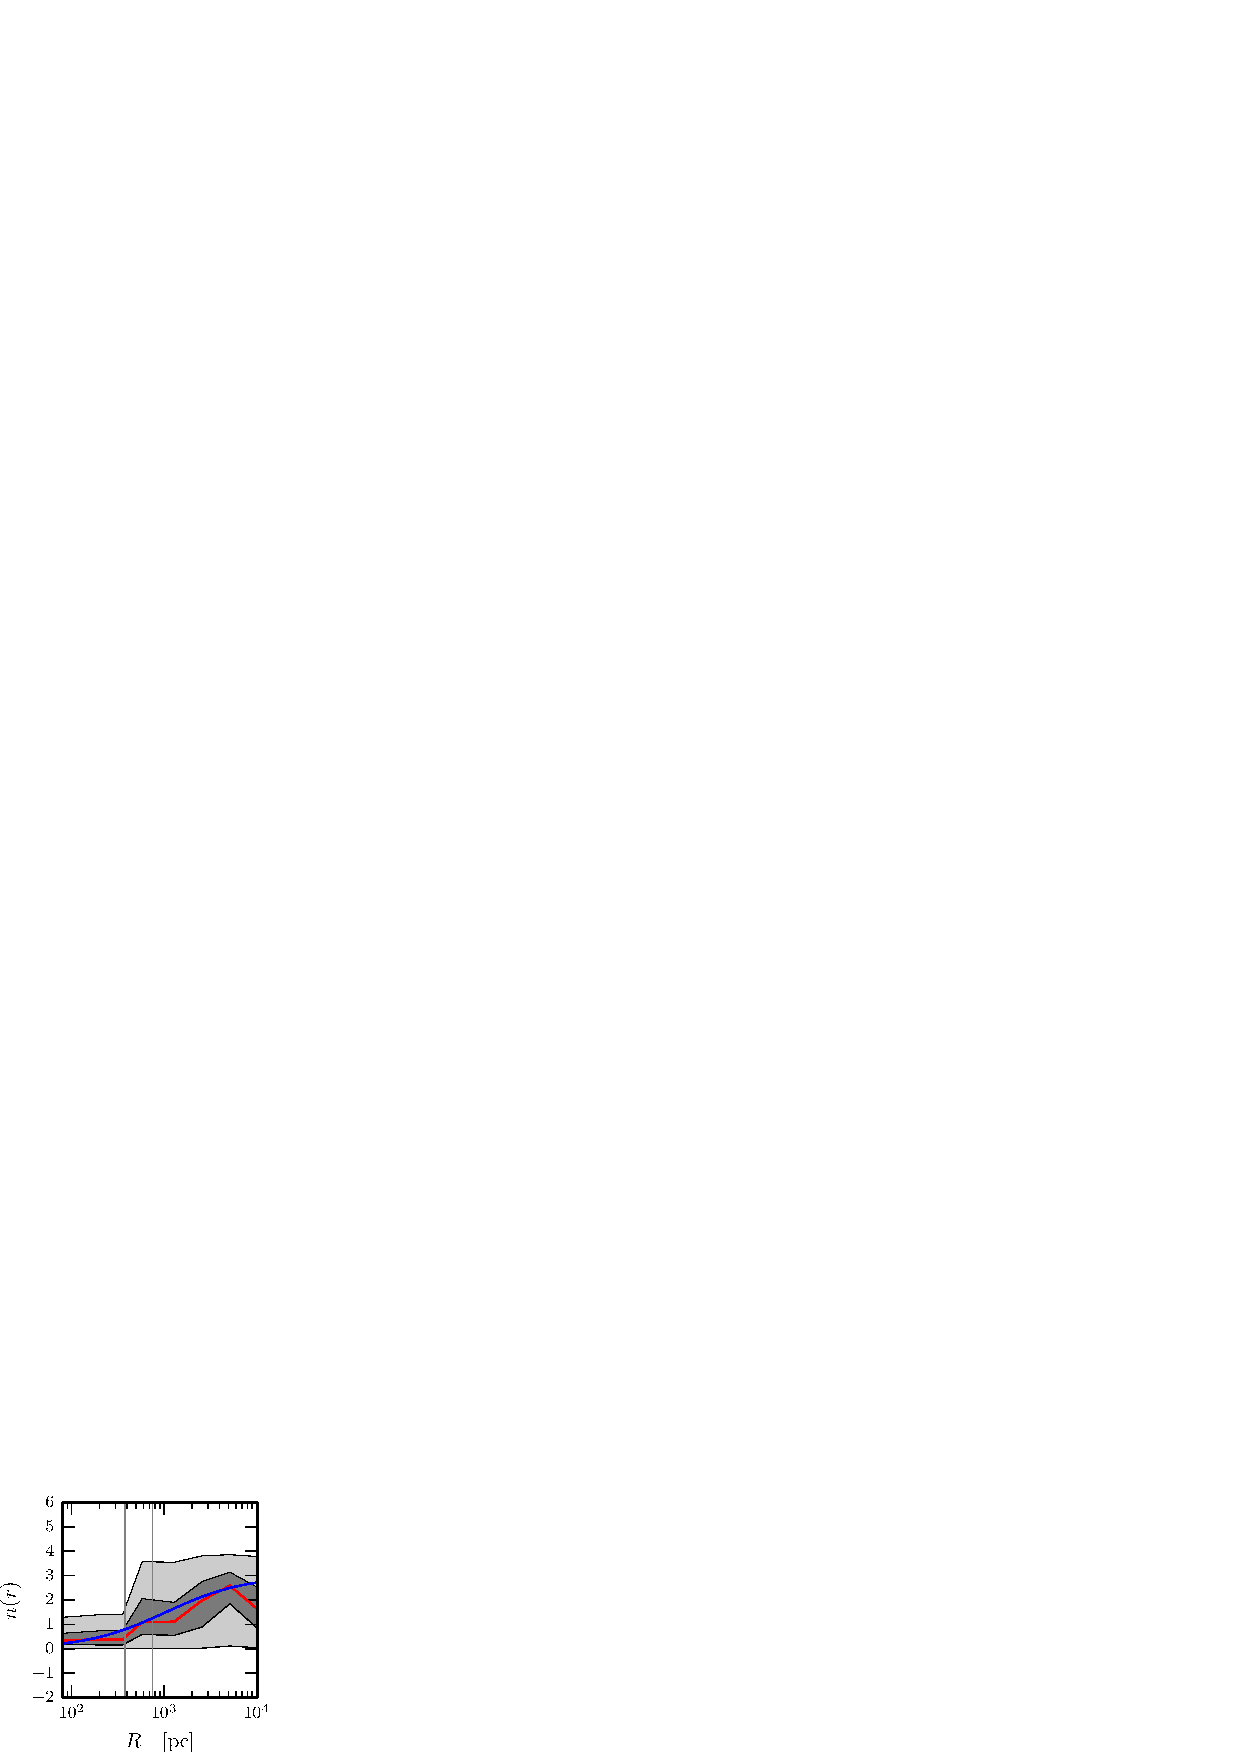
\includegraphics[width=0.3\textwidth]{fig/Triax01/output/pdf/prof_nr_0.pdf}
        \caption{Density profile of a cusped
          \TODO{triaxial} mock dwarf, for which the line
          of sight is inclined with 45 degrees
          with respect to all axes. The vertical
          line indicates the half-light radius at
          640pc.}
        \label{fig:triax}
    \end{center}
\end{figure*}

The retrieved density profile (fig. \ref{fig:triax}) recaptures the
density inside the half-light radius, but constantly overestimates it
at $r>r_{1/2}$. This is partly due to projection effects, as the
underlying density profile in blue is calculated for spherically
averaged density decrease.

\subsection{Data quality}
How many tracer stars are needed to determine the overall density profile
reliably? To address this question, we performed three runs with a restricted
set of tracer particles. In the first, $10^3$ particles were chosen out of the
$10^6$ simulated particles. With $10^4$ particles, the confidence intervals
shrink. These $10^4$ particles are then split into two populations of each
$5\cdot10^3$ particles, with different scalelengths of $r_S$ and $r_S/10$. Most
of the second population particles are inside the first two bins, so the overall
convergence is not visibly affected above the third bin.  However, the models
are better constrained around the scalelengths of both tracer populations. This
is expected from \citet{WalkerPenarrubia2011}, as any velocity anisotropy
sampling yields the same mass constraint there.

\begin{figure*}
    \begin{center}
        \hspace{-7mm}
        %\includegraphics[width=0.3\textwidth]{fig/hernquist1e3.pdf}
        %\includegraphics[width=0.3\textwidth]{fig/hernquist1e4.pdf}
        %\includegraphics[width=0.3\textwidth]{fig/hernquist2x5e3.pdf}
        \caption{\TODO{Hernquist} profile found by MCMC model (red) for $10^3$,
          $10^4$ and two times $5\cdot10^3$ tracer particles. The black curve
          shows the enclosed mass derived from the theoretical model.}
        \label{fig:hernquist1e3}
    \end{center}
\end{figure*}


%%% Local Variables:
%%% mode: latex
%%% TeX-master: "Steger_2014_Gravlite"
%%% End:
